
Knowledge of the availability of solar irradiance for energy conversion in a region
or specific location is central to solar energy applications. PV collectors are often
installed on inclined surfaces, either constrained by the tilt of roofs or intentionally
angled to maximize annual electricity production or shift peak generation to a desirable
time of day. However, irradiance data are mostly measured or estimated for horizontal
surfaces, necessitating the conversion of horizontal irradiance to in-plane values.
Models performing this task are known as transposition models.
The irradiance components on a horizontal surface are termed global horizontal
irradiance \(G_{\text{h}}\), diffuse horizontal irradiance \(D_{\text{h}}\), and beam or direct
horizontal irradiance \(B_{\text{h}}\). Analogously, \(G_{\text{c}}\), \(D_{\text{c}}\),
and \(B_{\text{c}}\) refer to in-plane values, where the subscript \say{c} stands
for \say{collector}. Transposition models have the general form:

\begin{align}
    G_{\text{c}} &= B_{\text{c}} + D_{\text{c}} + R_{\text{c}}
    \label{eq:In_plane_irradiance_total} \\[8pt]
    B_{\text{c}} &= B_{\text{h}} \, \frac{\cos \nu}{\cos \psi_{\text{s}}}
    \label{eq:In_plane_irradiance_beam} \\[0pt]
    R_{\text{c}} &= G_{\text{h}} \, \tau_{R} \, \rho = G_{\text{h}} \, \frac{1 - \cos \beta}{2} \, \rho
    \label{eq:In_plane_irradiance_reflected} \\[8pt]
    D_{\text{\text{c}}} &= D_{\text{h}} \, \tau_{D}
    \label{eq:In_plane_irradiance_diffuse}
\end{align}

\noindent
Here, \(\nu\) is the solar incidence angle, \(\psi_{\text{s}}\) is the solar zenith angle,
\(\beta\) is the surface tilt angle as discussed in Section \ref{sec:Solar Geometry},
\(\rho\) is the albedo quantifying the ground's reflectivity, and \(\tau_{D}\) and \(\tau_{R}\)
are transposition factors for the diffuse and reflected components, respectively
\cite[p. 1f]{Quan2020}. As expected from the previous section, the global tilted
irradiance in Equation \ref{eq:In_plane_irradiance_total} is modeled as the sum
of the three irradiance components: beam, diffuse, and reflected.

The beam component in Equation \ref{eq:In_plane_irradiance_beam} follows a geometric
relation where the second factor adjusts the horizontal value \(B_{\text{h}}\). The latter can be
calculated as the difference between horizontal global irradiance \(G_{\text{h}}\) and diffuse
irradiance \(D_{\text{h}}\) \cite[p. 144]{Muneer}. To understand the formula, let \(B_{\text{n}}\) denote
the direct normal irradiance received by a surface perpendicular to the sun's rays.
The in-plane beam irradiance B received by any surface with incidence angle \(\nu\), 
assuming parallel sun rays, is expressed as:

\begin{equation}
    B = B_{\text{n}} \cos \nu
    \label{eq:In_plane_beam_irradiance_derivation}
\end{equation}

\noindent
This equation implies that a surface tilted away from the sun's rays by angle \(\nu\)
receives only a fraction of the direct normal radiation \(B_{\text{n}}\), given by \(\cos \nu\).
This fraction equals the proportion of the surface's projection onto a plane perpendicular
to the sun rays. Figure \ref{fig:In_plane_beam_irradiance_derivation_visualization}
illustrates this derivation. Application of Equation \ref{eq:In_plane_beam_irradiance_derivation}
to a horizontal and a tilted surface, denoted by subscripts \say{h} and \say{c} respectively,
yields:

\begin{align}
    B_{\text{h}} &= B_{\text{n}} \cos \psi_{\text{s}} \\[7pt]
    B_{\text{c}} &= B_{\text{n}} \cos \nu \\[4pt]
    \Rightarrow B_{\text{c}} &= B_{\text{h}} \, \frac{\cos \nu}{\cos \psi_{\text{s}}}
\end{align}

\noindent
where in the case of a horizontal surface, \(\nu = \psi_{\text{s}}\).

As mentioned in \cite{SandiaNationalLaboratory}, the ground-reflected irradiance on a tilted
surface \(R_{\text{c}}\) is calculated based on the irradiance on the ground, the ground's reflectivity
\(\rho\), and the surface tilt angle \(\beta\). Equation \ref{eq:In_plane_irradiance_reflected} assumes,
among other things, that the ground irradiance is uniform, equal to \(G_{\text{h}}\) and reflected equally
in all directions, that is, the ground acts as a Lambertian reflector. These idealized assumptions,
resulting in the common transposition factor \(\tau_{R} = \frac{1 - \cos \beta}{2}\), are widely used
in transposition calculations despite their limitations \cite{Gueymard2017, Quan2020}. Table
\ref{tab:Reflected_in_plane_irradiance_transposition_factor_for_different_surface_tilts}
summarizes how the ground transposition factor and the reflected component change with different surface tilts.
As the tilt angle increases, the surface starts to \say{see} more of the ground and receives therefore more
ground-reflected irradiance. The transposition factor smoothly transitions between 0 and \(\frac{1}{2}\)
as \(\beta\) varies from \(0^\circ\) to \(90^\circ\). Equation \ref{eq:In_plane_irradiance_reflected}
uses a constant albedo value. Figure \ref{fig:Albedo_variability} illustrates the variability of
measured reflectivity at a station in Murcia, Spain, during representative days in winter and summer, as well as throughout the year.
Clearly, assuming a constant albedo is idealistic and can increase the transposition model's error.
Unfortunately, accurate information on a site's surroundings is rarely available. The PVsyst
modeling software provides guidance for estimating albedo values, as presented in Table
\ref{tab:Sandia_National_Laboratories_albedo}.

\begin{table}
    \centering
    \begin{tabular}{ll}
        \toprule
        \textbf{Surface} & \textbf{Albedo \(\rho\)} \\
        \midrule
        Urban environment & 0.14-0.22 \\
        Grass & 0.15-0.25 \\
        Fresh grass & 0.26 \\
        Fresh snow & 0.82 \\
        Wet snow & 0.55-0.75 \\
        Dry asphalt & 0.09-0.15 \\
        Wet asphalt & 0.18 \\
        Concrete & 0.25-0.35 \\
        Red tiles & 0.33 \\
        Aluminum & 0.85 \\
        Copper & 0.74 \\
        New galvanized steel & 0.35 \\
        Very dirty galvanized steel & 0.08 \\
        \bottomrule
    \end{tabular}
    \caption{\small Estimates of ground albedo values for various surfaces \cite{SandiaNationalLaboratory}.}
    \label{tab:Sandia_National_Laboratories_albedo}
\end{table}

\begin{figure}
    \centering
    \subfloat[\centering]{{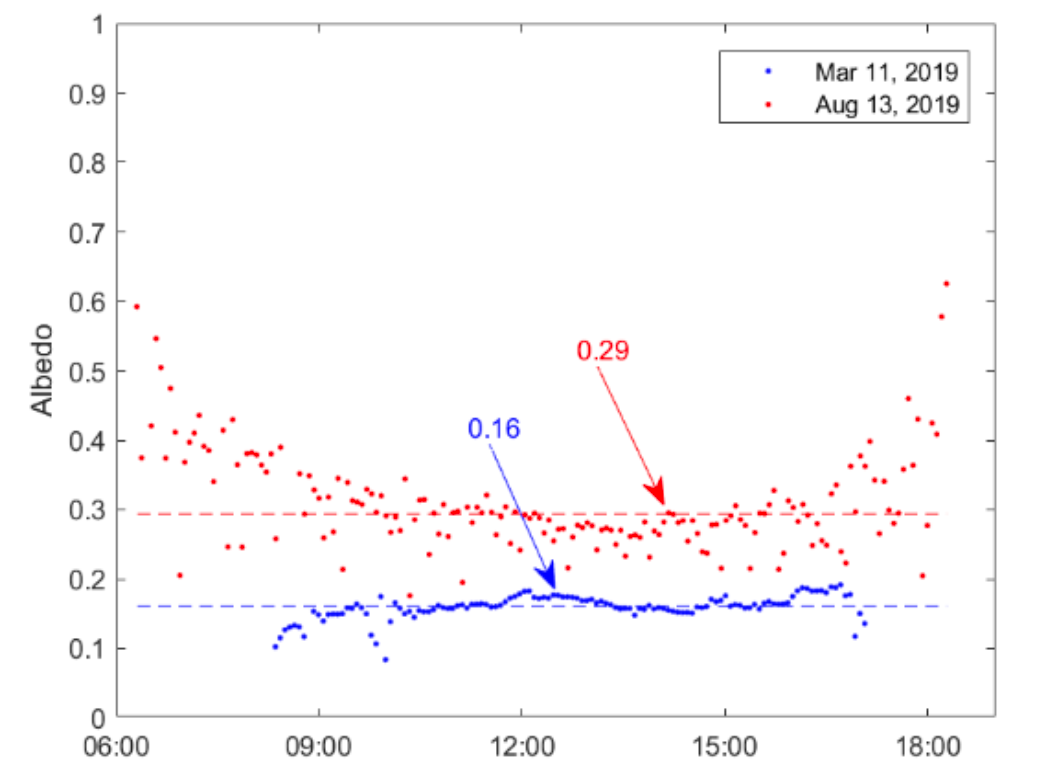
\includegraphics[width=7.1cm]{Albedo_variability_throughout_the_year.png} }}
    \qquad
    \subfloat[\centering]{{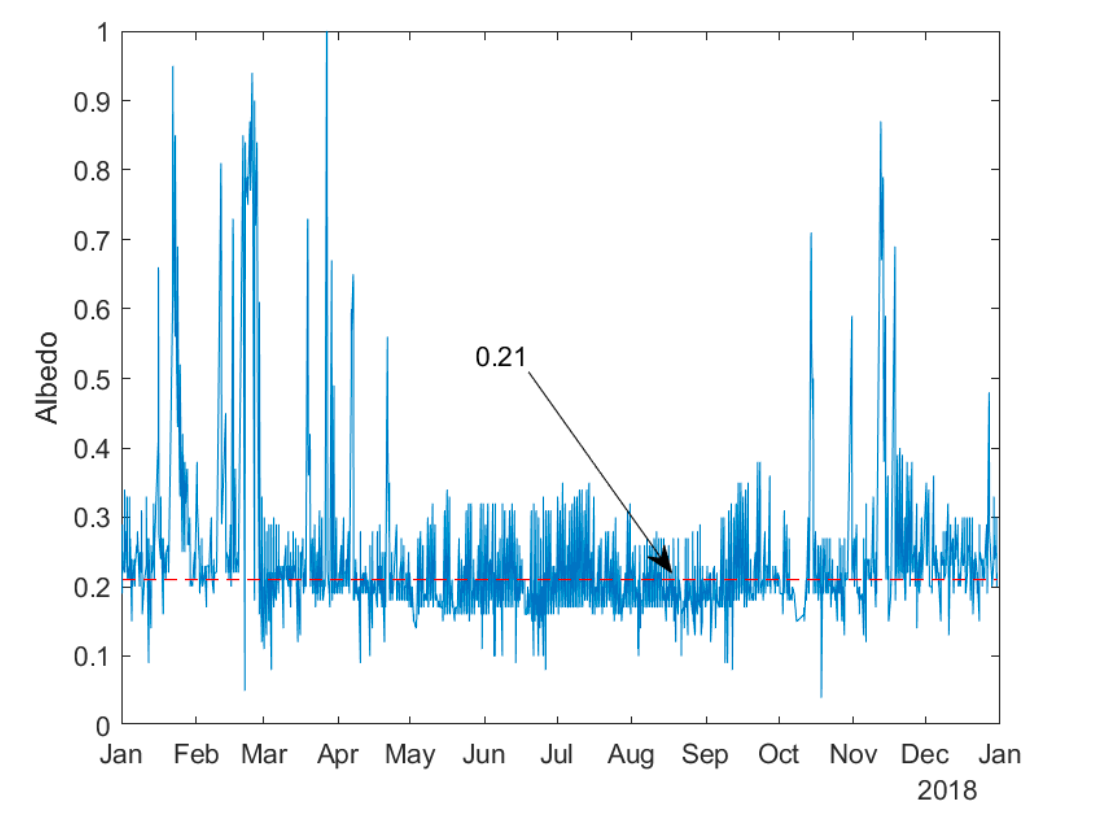
\includegraphics[width=7cm]{Albedo_variability_on_two_days.png} }}
    \caption{\small Variability of albedo during the day a) and throughout the year b) with indication
        of median values \cite{Toledo}.}
    \label{fig:Albedo_variability}
\end{figure}

\begin{table}
    \centering
    \renewcommand{\arraystretch}{1.25}
    \begin{tabular}{lll}
        \toprule
        \textbf{Surface tilt} \(\beta\) & \textbf{Transposition factor} \(\tau_{R} \)& \textbf{Reflected component} \(R_{\text{c}}\) \\
        \midrule
        \(0^\circ\) & 0 & 0  \\
        \(90^\circ\) & \(\frac{1}{2}\) & \(G_{h} \rho \frac{1}{2}\) \\
        \(\beta \in (0^\circ, 90^\circ)\) & \(\frac{1 - \cos \beta}{2} \in (0, \frac{1}{2})\) & \(G_{h} \: \rho \: \frac{1 - \cos \beta}{2}\) \\
        \bottomrule
    \end{tabular}
    \caption{\small Equation \ref{eq:In_plane_irradiance_reflected} for different surface tilts.}
    \label{tab:Reflected_in_plane_irradiance_transposition_factor_for_different_surface_tilts}
\end{table}

\begin{figure}
    \centering
    \begin{tabular}{@{}cc@{}}
        \begin{tikzpicture}
            \coordinate (center) at (3,0);
            \coordinate (left) at (0,0);
            \coordinate (right) at (6,0);
            \coordinate (top) at (3,3);
            \coordinate (A) at (0.401923788646684,1.4999999999999998);
            \coordinate (A_inside) at (1.2679491924311226, 0.9999999999999999);
            \coordinate (B) at (1.5000000000000007,2.598076211353316);
            \coordinate (B_inside) at (2.5, 0.8660254037844387);
            \coordinate (C) at (3.0179491924311224, 4.031088913245535);
            \coordinate (D) at (5.531088913245536, 2.6160254037844384);

            \draw (0,0) -- (6,0) node[above, near end, black, xshift = -0.5pt] {\tiny horizontal plane};
            \draw[thick] (center) -- (A) node[pos = 1, above, black] {\tiny surface};
            \draw (A_inside) -- (C) node[at end, black, above] {\tiny normal to surface};
            \draw[dashed, thick, black] (center) -- (B);
            \draw[dashed, black] (B_inside) -- (D) node[at end, above, black] {\tiny shifted normal};

            \pic [draw, <-, angle radius=1.5cm, "$\nu$", black] {angle = B--center--A};
        \end{tikzpicture} & 
        \begin{tikzpicture}
            \coordinate (center) at (3,0);
            \coordinate (left) at (0,0);
            \coordinate (right) at (6,0);
            \coordinate (top) at (3,3);

            \coordinate (A) at (0.401923788646684,1.4999999999999998);
            \coordinate (A_inside) at (1.2679491924311226, 0.9999999999999999);
            \coordinate (B) at (1.5000000000000007,2.598076211353316);
            \coordinate (B_inside) at (2.5, 0.8660254037844387);
            \coordinate (C) at (3.7679491924311224,5.330127018922193);
            \coordinate (D) at (6.830127018922194, 3.3660254037844384);

            \coordinate (E) at (3.866025403784439, 3.4999999999999996);
            \coordinate (F) at (6.464101615137755, 1.9999999999999998);
            \coordinate (G) at (1.7009618943233424, 2.2500000000000004);

            \draw (0,0) -- (6,0);
            \draw (0,0) arc[start angle=180, end angle=0, radius=3cm];
            \draw[thick] (center) -- (A);
            \draw[dashed, black] (center) -- (B);        
            \draw[dashed, thick, black] (A) -- (E) node[pos=1, yshift = -3pt, above, black] {\tiny Sun rays || shifted normal};
            \draw[dashed, thick, black] (center) -- (F) node[midway, above, sloped, black] {\tiny Sun ray};
            \draw[thick] [decorate, decoration = {calligraphic brace, amplitude = 7pt, mirror}] (center) -- (G) node[midway, above, sloped, black, yshift = 5pt] {\tiny $\cos \nu$};
            
            \pic [draw, <-, angle radius=1.5cm, "$\nu$", black] {angle = B--center--A};
        \end{tikzpicture} \\ (a) \: \: & (b) \: \:
    \end{tabular}
    \caption{\small Visualization of the relation between the beam irradiance received
        by a perpendicular surface and a surface with incidence angle \(\nu\).}
    \label{fig:In_plane_beam_irradiance_derivation_visualization}
\end{figure}

The interaction of solar radiation with the atmosphere results in the diffuse component 
\(D_{\text{c}}\) mentioned in Section \ref{sec:Irradiance and Radiation}. On one hand, it is subject
to attenuation and absorption by atmospheric molecules such as water vapor (H$_2$O), ozone
(O$_3$), and carbon dioxide (CO$_2$). On the other hand, it is scattered by molecules like
nitrogen (N$_2$) and oxygen (O$_2$) distributed throughout the sky dome. Figure
\ref{fig:Absorption_of_solar_radiation} shows the absorption of shortwave radiation
due to various atmospheric constituents, indicated by dips in the curves.
From a modeling perspective, two types of transposition models exist:
isotropic and anisotropic. These models assume a uniform versus non-uniform
distribution of the diffuse component over the sky, respectively \cite[p. 5]{Toledo}.
The interactions between atmospheric molecules and radiation suggest that an isotropic
model may be too inaccurate for the diffuse component, a notion confirmed by several
comparison studies \cite{Hay1985, PerezDriesse2024}. Numerous transposition models
are documented in the literature, along with abundant evaluation studies. The
comprehensive study by Yang et al. \cite{Yang2016} analyzed the accuracy of 26
transposition models using one year of solar irradiance measurements from four
locations. Although no universal model outperformed all others in every case study,
some were recommended. These include the family of Perez models, particularly a
representative version described in the remainder of this section.

The first version of the anisotropic Perez model \cite{Perez1986} divided the sky hemisphere
into three zones to account for the main anisotropy observed in the atmosphere: circumsolar
brightening due to forward scattering by aerosols and horizon brightening primarily due to
multiple Rayleigh scattering and backscattering in clear atmospheres. Figure \ref{fig:Perez_sky_dome}
shows the geometrical representation of these three zones. The circumsolar region is a
reversed cone with a radius \(\alpha = 15^\circ\), centered on the Sun's position, and the
horizon band is defined by an angular thickness \(\zeta = 6.5^\circ\).
The authors derived the model's governing equation from two expressions that describe how
the horizontal diffuse irradiance and the irradiance received by a tilted surface can be
calculated under the assumption that the radiances originating from the main portion of
the dome, the circumsolar region, and the horizon zone are respectively equal to \(L\), \(F_{1} L\),
and \(F_{2} L\). The products are indicated as \(F_{i} \times L\) in the illustration. The
non-dimensional coefficients \(F_{1}\) and \(F_{2}\) were the only undefined terms in
the model's equation. Least-squares fitting of measured data on sloped surfaces from
four sites with different climatic conditions was performed to obtain values for these
coefficients across 240 sky condition categories \cite[p. 481ff]{Perez1986}.
The next publication on the model \cite{Perez1987} aimed to simplify the model while maintaining or improving
its accuracy. A major simplification was rewriting the governing equation in terms of reduced
brightness coefficients, allowing for negative values to cover a broader range of sky conditions.
Additional simplifications included treating the horizon band as an infinitesimally thin region
at 0° elevation and considering the circumsolar energy as originating from a point source.
\cite[p. 222ff]{Perez1987}. Building upon these simplifications, the point source version of the model, as presented
in \cite{Perez1990}, is based on the previous considerations and is the version employed in this thesis.
This model estimates the incident diffuse energy on any tilted surface using the following equation:

\begin{figure}
    \centering
    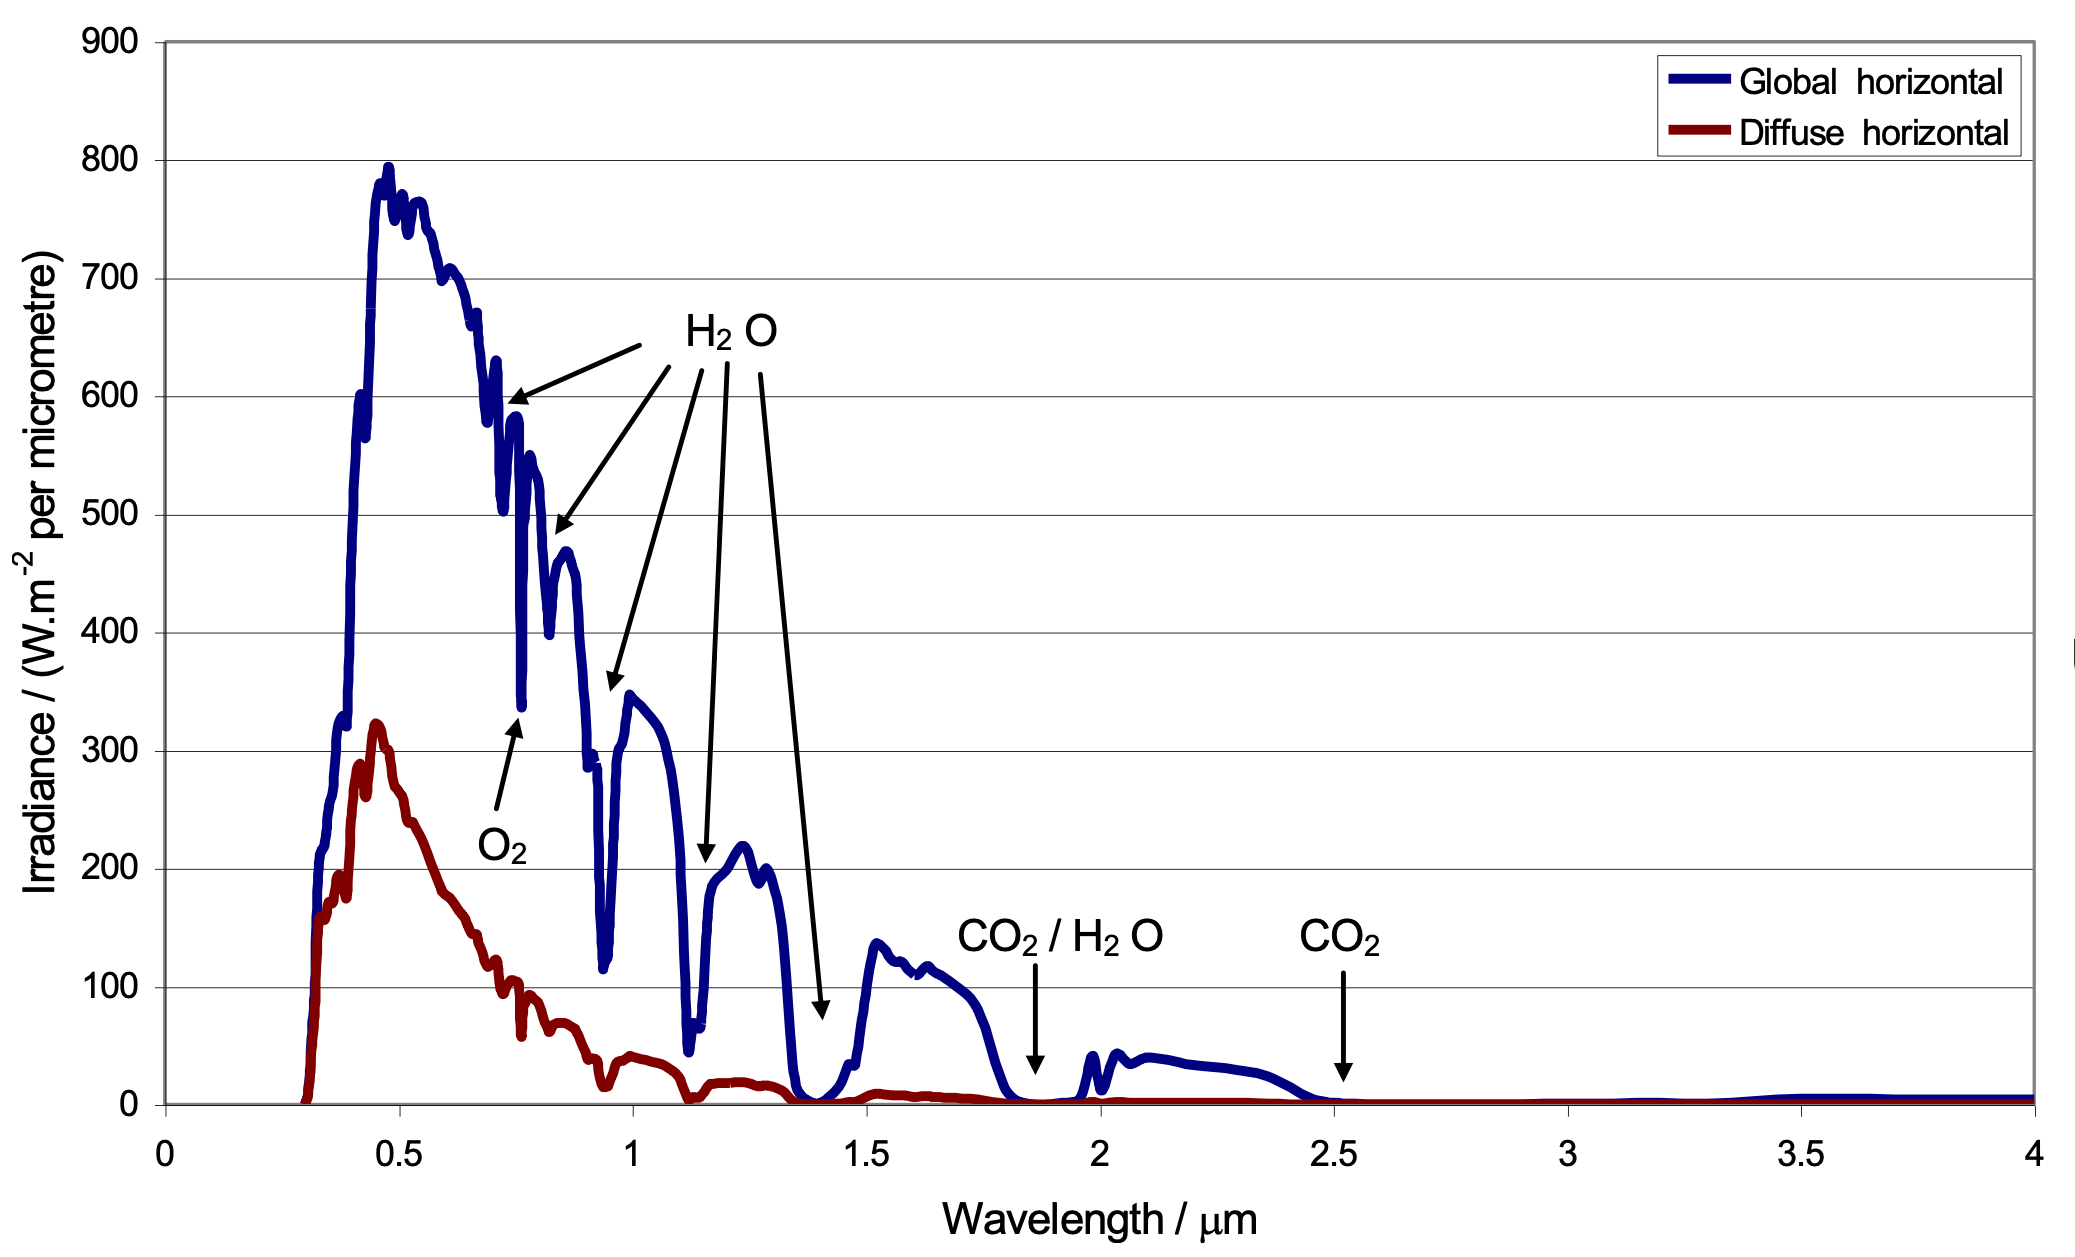
\includegraphics[scale=0.17]{Solar_Geometry_absorption_of_solar_radiation.png}
    \caption{\small Absorption of radiation due to various atmospheric constituents \cite{CIBSE}.}
    \label{fig:Absorption_of_solar_radiation}
\end{figure}

\begin{figure}
    \centering
    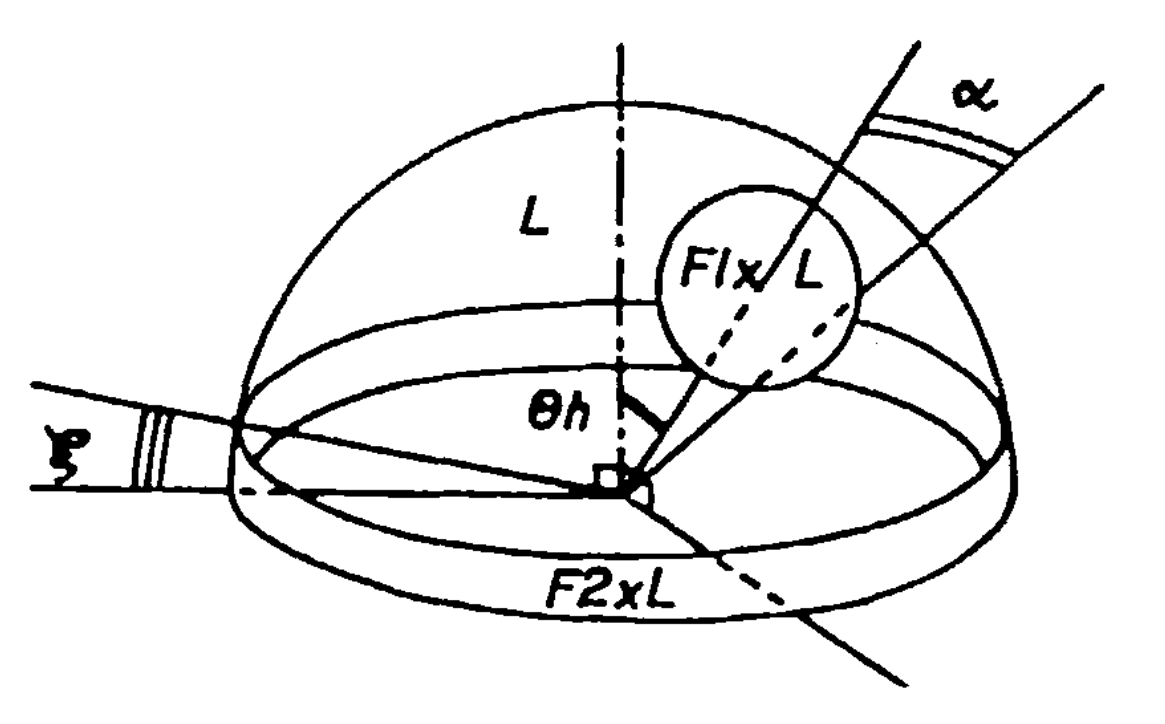
\includegraphics[scale=0.23]{Perez_sky_dome.png}
    \caption{\small Geometrical representation of the sky dome in Perez's slope irradiance model \cite{Perez1986}.}
    \label{fig:Perez_sky_dome}
\end{figure}

% \begin{table}[H]
%     \centering
%     \begin{tabular}{l|c|c|c|l}
%         \toprule
%         Station & Latitude & Longitude & Elevation & Climate Type \\
%         \midrule        
%         Albany, New York & 42° 42'N & 73° 50'W & 94m & Humid \\
%         &          &           &     & Continental \\
%         &          &           &     & Temperate \\
%         San Antonio, Texas & 29° 46'N & 98° 49'W & 253m & Semi-arid \\
%                 &          &           &      & Sub tropical \\
%         Carpentras, France & 44° 05'N & 5° 03'E & 99m & Mediterranean \\
%         Trappes, France & 48° 46'N & 2° 0'E & 167m & Marine \\
%             &          &         &      & Temperate \\
%         \bottomrule
%     \end{tabular}
%     \caption{Description of selected sites \cite{Perez1986}.}
%     \label{tab:Perez1986_sites}
% \end{table}

\begin{equation}
    D_{\text{c}} = D_{\text{h}} \: \biggl[ (1-F_{1}) \: \frac{1 + \cos \beta}{2} + F_{1}\frac{a}{b} + F_{2} \sin\beta\biggr]
    \label{eq:Perez_in_plane_irradiance}
\end{equation}

\noindent
Here, the second factor on the right side is the diffuse transposition factor \(\tau_{D}\)
from Equation \ref{eq:In_plane_irradiance_diffuse}. The terms \(a\) and \(b\) account for the 
angles of incidence of circumsolar radiation on the tilted and horizontal surfaces, 
respectively:

\begin{align}
    a &= \max\{0, \cos\nu\} \\
    b &= \max\{\cos85^\circ, \cos \psi_{\text{s}}\}
\end{align}

\noindent
The anisotropic coefficients \(F_{1}\) and \(F_{2}\) express the degree of circumsolar and horizon anisotropy,
respectively. They are functions of the sky conditions, characterized by the solar zenith angle
\(\psi_{\text{s}}\), the clearness index \(\epsilon\), and the brightness index \(\Delta\):

\begin{align}
    F_{1} &= \min \Bigl\{ 0.9, \max\bigl\{0, f_{11}(\epsilon) + f_{12}(\epsilon)\Delta + \frac{\pi \psi_{\text{s}}}{180}f_{13}(\epsilon) \bigr\} \Bigr\}
    \label{eq:brightness_coefficient_circumsolar} \\
    F_{2} &= f_{21}(\epsilon) + f_{22}(\epsilon)\Delta + \frac{\pi \psi_{s}}{180}f_{23}(\epsilon)
    \label{eq:brightness_coefficient_horizon}
\end{align}

\noindent
Following recommendations from \cite{PerezDriesse2024}, a limit of 0.9 is imposed on \(F_{1}\) to
ensure physically coherent results. The clearness index \(\epsilon\) is calculated as:

\begin{equation}
    \epsilon = \frac{\bigl(\frac{D_{\text{h}} + B_{\text{n}}}{D_{\text{h}}}\bigl) + 5.535\cdot10^{-6} \psi_{\text{s}}^3}{1 + 5.535\cdot10^{-6} \psi_{\text{s}}^{3}}
\end{equation}

\noindent
The brightness index \(\Delta\) is given by:

\begin{equation}
    \Delta = m_{\text{air}} \, \frac{D_{\text{h}}}{G_{\text{e}}}
\end{equation}

\noindent
where \(m_{\text{air}}\) is the air mass and \(G_{\text{e}}\) is the extraterrestrial normal irradiance.
As referenced in \cite{Toledo}, the air mass can be calculated using the empirical
equation by Kasten and Young \cite{Karsten}:

\begin{equation}
    m_{\text{air}} = \frac{\exp(-0.0001184h)}{\cos(\psi_{\text{s}}) + 0.5057(96.080 - \psi_{\text{s}})^{-1.634}}
\end{equation}

\noindent
Here, \(h\) is the site altitude in meters. The extraterrestrial irradiance is calculated using 
Spencer's formula \cite{Spencer1971Fourier}, with an accuracy of \(\pm0.01\%\):

\begin{align}
    G_{\text{e}} = 1367 \: \bigl(&1.00011 + 0.034221 \cos Q + 0.00128 \sin Q \nonumber \\ 
                     &+ 0.000719 \cos 2Q + 0.000077 \sin2Q\bigr)
\end{align}

\noindent
where 1367 is the solar constant (\si{\watt\per\square\meter}) and \(Q\) is given by:

\begin{equation}
    Q = (n_{\text{day}} - 1) \frac{360}{365}
\end{equation}

\noindent
with \(n_{\text{day}}\) being the nth day of the year. A recommended set of coefficients for
calculating the brightness coefficients in Equations \ref{eq:brightness_coefficient_circumsolar}
and \ref{eq:brightness_coefficient_horizon} is provided in Table
\ref{tab:Perez_coeff}. These coefficients were fitted using data
from 10 American and three European cities covering different climatic
environments. Table \ref{tab:Perez_experimental_data} summarizes the
climatic environments and datasets used.
The discrete sky clearness categories range from overcast in the first
row to clear in the last row \cite[p. 273]{Perez1990}. These coefficients
could be fitted to a local climate if high-quality datasets of measured
sloped irradiance for different orientations, along with corresponding
meteorological data, are available. 

\begin{table}
    \resizebox{\columnwidth}{!}{
        \begin{tabular}{c S S S S S S}
            \toprule
            Sky clearness \(\epsilon\) & {$f_{11}$} & {$f_{12}$} & {$f_{13}$} & {$f_{21}$} & {$f_{22}$} & {$f_{23}$} \\
            \midrule
            $[1.000, 1.065)$ & -0.0083 & 0.5877 & -0.0621 & -0.0596 & 0.0721 & -0.0220 \\
            $[1.065, 1.230)$ & 0.1299  & 0.6826 & -0.1514 & -0.0189 & 0.0660  & -0.0289 \\
            $[1.230, 1.500)$ & 0.3297  & 0.4869 & -0.2211 & 0.0554  & -0.0640 & -0.0261 \\
            $[1.500, 1.950)$ & 0.5682  & 0.1875 & -0.2951 & 0.1089  & -0.1519 & -0.0140 \\
            $[1.950, 2.800)$ & 0.8730   & -0.3920 & -0.3616 & 0.2256  & -0.4620  & 0.0012 \\
            $[2.800, 4.500)$ & 1.1326  & -1.2367 & -0.4118 & 0.2878 & -0.8230  & 0.0559 \\
            $[4.500, 6.200)$ & 1.0602  & -1.5999 & -0.3589 & 0.2642 & -1.1272 & 0.1311 \\
            $[6.200, \infty)$ & 0.6777  & -0.3273 & -0.2504 & 0.1561 & -1.3765 & 0.2506 \\
            \bottomrule
        \end{tabular}
    }
    \caption{\small Coefficients for Perez slope irradiance model \cite[Ch.\ 4]{Muneer}.}
    \label{tab:Perez_coeff}
\end{table}

\begin{table}[H]
    \centering
    \resizebox{\columnwidth}{!}{
        \begin{tabular}{lll}
            \toprule
            \textbf{Site} & \textbf{Main Environmental Fatures} & \textbf{Span and Frequency} \\
            \midrule
            Geneva, & Temperate maritime, with central Europe & 1 yr. hourly data \\
            Switzerland & continental influence. Persistent &  \\
            & nebulosity enhanced by blocking position &  \\
            & at foot-hill of the Alps. &  \\
            % \midrule
            % & & \\
            Trappes, & Temperate maritime with high incidence of & 3 yr. hourly data \\
            France & intermediate skies. &  \\
            % \midrule
            % & & \\
            Carpentras, & Mediterranean & 3 yr. hourly data \\
            France & & \\
            % \midrule
            % & & \\
            Albany, & Humid continental with bimodal influence & 3 yr. hourly data \\
            NY, USA & & 2 yr. 15 min. data \\
            % \midrule
            % & & \\
            New York, & Humid continental with maritime influence & 1 yr. 15 min. data \\
            NY, USA & plus large city's anthropogenic environment &  \\
            % \midrule
            % & & \\
            Farmingdale, & Same as above but without city's environment & 1 yr. 15 min. data \\
            NY, USA & & \\
            % \midrule
            % & & \\
            Oswego, & Humid continental, Great Lakes basin & 6 mo. 15 min. data \\
            NY, USA & & \\
            % \midrule
            % & & \\
            Glens Falls, & Humid continental & 6 mo. 15 min. data \\
            NY, USA & & \\
            % \midrule
            % & & \\
            Phoenix, & Arid, low elevation & 6 mo. hourly data \\
            AZ, USA & & \\
            % \midrule
            % & & \\
            Albuquerque, & Arid, high elevation (1800 m) & 1 yr. hourly data \\
            NM, USA & & \\
            % \midrule
            % & & \\
            Los Angeles, & Arid and maritime influence plus high & 6 mo. hourly data \\
            CA, USA & frequency of anthropogenic smog events &  \\
            % \midrule
            % & & \\
            Osage, & Continental, U.S. Great Plains & 6 mo. hourly data \\
            KS, USA & & \\
            % \midrule
            % & & \\
            C. Canaveral, & Subtropical, low latitude, maritime & 6 mo. hourly data \\
            FL, USA & & \\
            \bottomrule
        \end{tabular}
    }
    \caption{\small Origin, size, and climatic environment of experimental data sets \cite{Perez1990}.}
    \label{tab:Perez_experimental_data}
\end{table}

% \begin{figure}
%     \centering
%     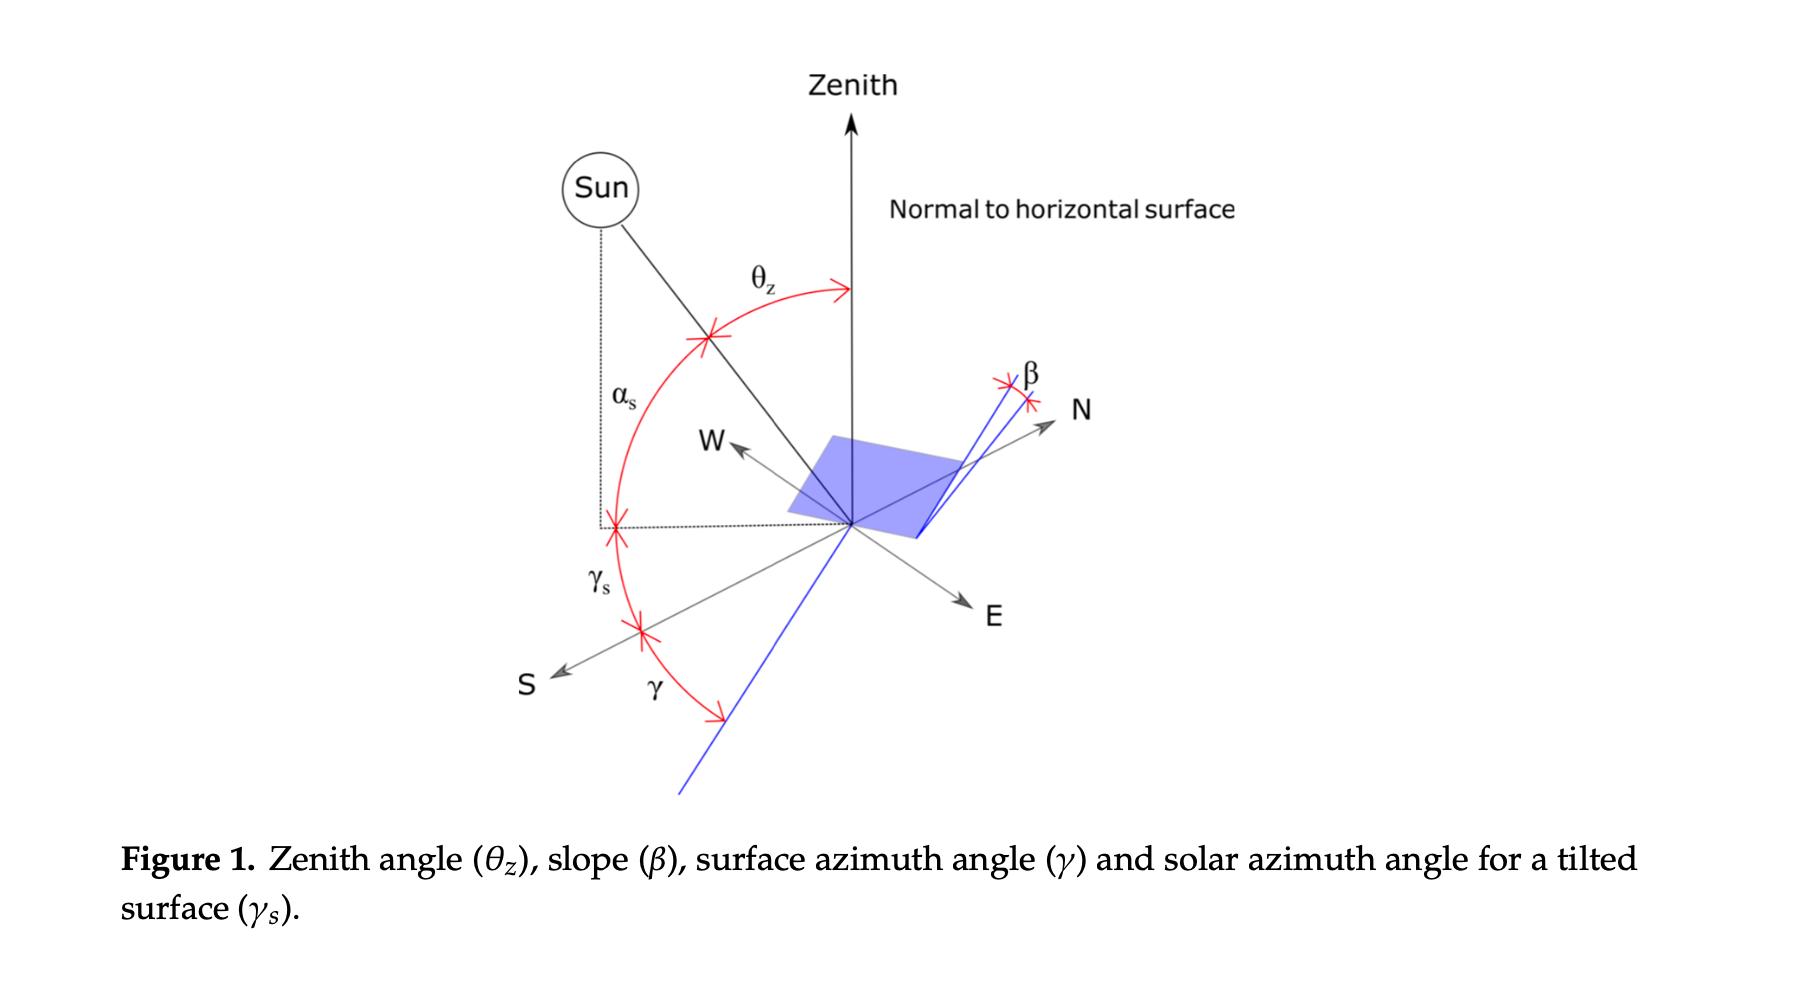
\includegraphics[scale=0.23]{Solar_Geometry_Toledo.png}
%     \caption{Solar geometry here just as a reference during thesis developement \cite{CIBSE}.}
% \end{figure}